
\documentclass{standalone}
\usepackage{tikz}
\usepackage{circuitikz}

\begin{document}
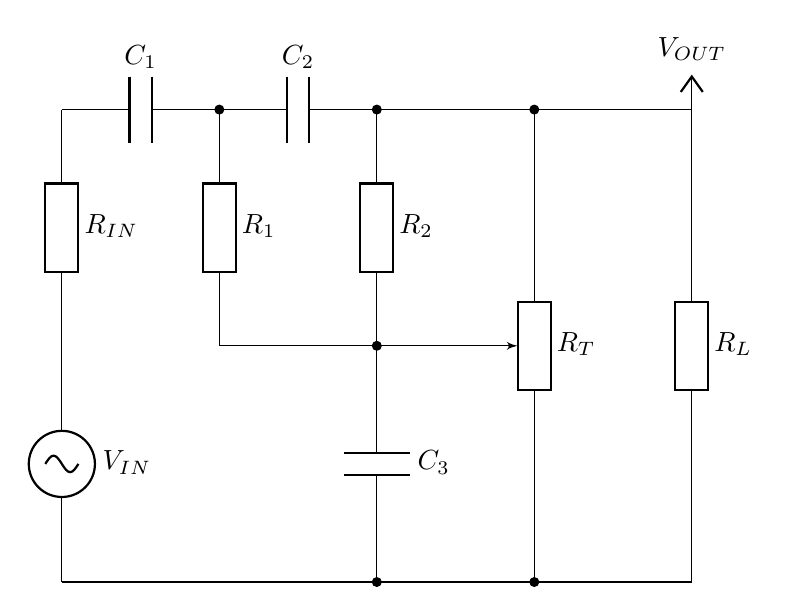
\begin{tikzpicture}
	\draw (2, 7) to[sinusoidal voltage source, l=$V_{IN}$] (2, 4);

	\draw (2, 10) to[european resistor, l=$R_{IN}$] (2, 7);
	\draw (4, 10) to[european resistor, l=$R_1$] (4, 7);
	\draw (6, 10) to[european resistor, l=$R_2$] (6, 7);
	\draw (10, 10) to[european resistor, l=$R_L$] (10, 4);

	\draw (8, 4) to[european potentiometer, l_=$R_T$] (8, 10);

	\draw (2, 10) to[capacitor, l=$C_1$] (4, 10);
	\draw (4, 10) to[capacitor, l=$C_2$] (6, 10);
	\draw (6, 7) to[capacitor, l=$C_3$] (6, 4);

	\draw (2, 4) -- (10, 4);
	\draw (4, 7) -- (7.44, 7);
	\draw (6, 10) -- (10, 10);

	\node[vcc] at (10, 10) {$V_{OUT}$};
	\node[circ] at (4, 10) {};
	\node[circ] at (6, 10) {};
	\node[circ] at (6, 4) {};
	\node[circ] at (6, 7) {};
	\node[circ] at (8, 10) {};
	\node[circ] at (8, 4) {};

\end{tikzpicture}
\end{document}